\begin{figure}
	\centering 
	\begin{tabular}{c}
		\raisebox{-0.3cm}{Input} \\ 
		\raisebox{-2.3cm}{3-D Pose}
	\end{tabular} 
	\begin{subfigure}[t]{0.18\linewidth} \centering
		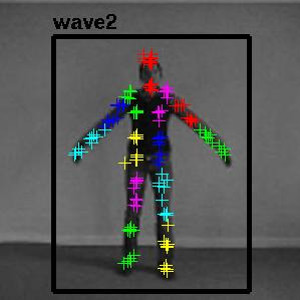
\includegraphics[height=2.3cm]{fig/body/others/kth3.jpg} \\
		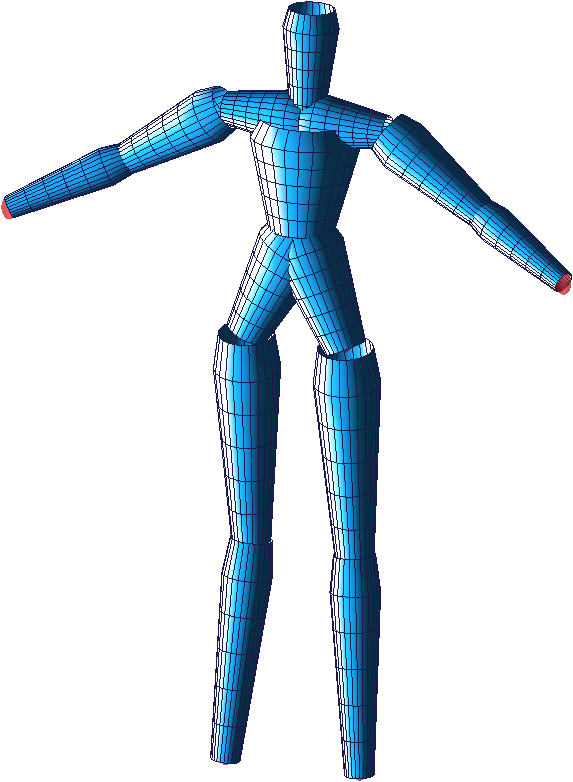
\includegraphics[height=2.3cm]{fig/body/others/kth3.png} 
		\subcaption{Wave 2}
		\label{fig/body/others/a}
	\end{subfigure}
	\begin{subfigure}[t]{0.18\linewidth} \centering
		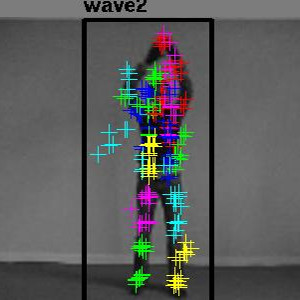
\includegraphics[height=2.3cm]{fig/body/others/kth1.jpg} \\
		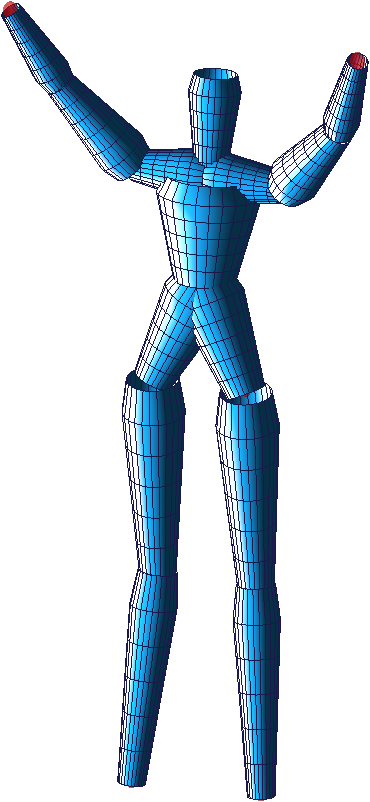
\includegraphics[height=2.3cm]{fig/body/others/kth1.png} 
		\subcaption{Wave 2}
		\label{fig/body/others/b}
	\end{subfigure}
	\begin{subfigure}[t]{0.18\linewidth} \centering
		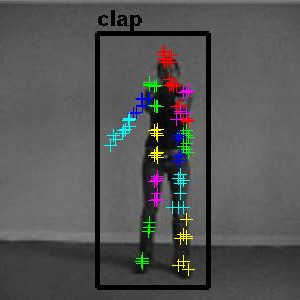
\includegraphics[height=2.3cm]{fig/body/others/kth2.jpg} \\
		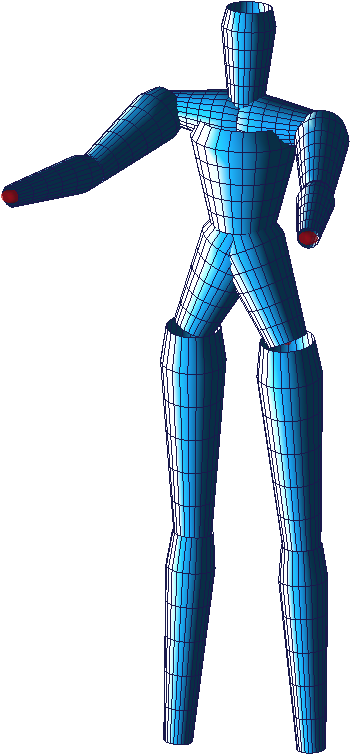
\includegraphics[height=2.3cm]{fig/body/others/kth2.png} 
		\subcaption{Clap}
		\label{fig/body/others/c}
	\end{subfigure}
	\begin{subfigure}[t]{0.18\linewidth} \centering
		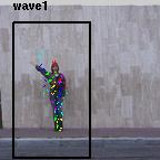
\includegraphics[height=2.3cm]{fig/body/others/weiz3.jpg} \\
		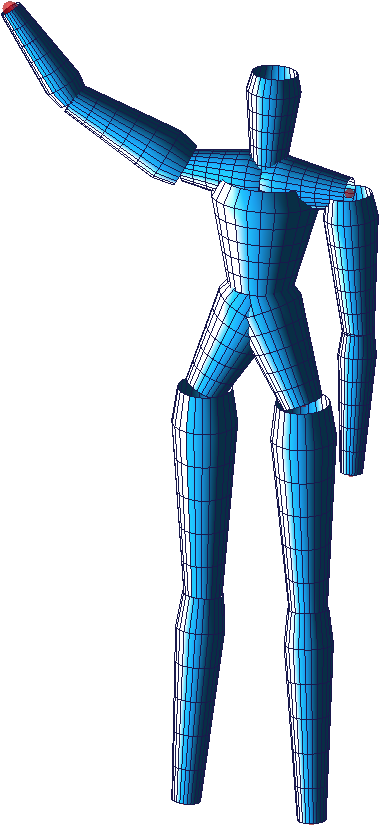
\includegraphics[height=2.3cm]{fig/body/others/weiz3.png} 
		\subcaption{Wave 1}
		\label{fig/body/others/d}
	\end{subfigure} \\ 
	\begin{tabular}{c}
		\raisebox{-0.3cm}{Input} \\ 
		\raisebox{-2.3cm}{3-D Pose}
	\end{tabular} 
	\begin{subfigure}[t]{0.18\linewidth} \centering
		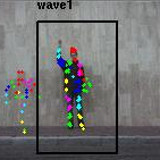
\includegraphics[height=2.3cm]{fig/body/others/weiz1.jpg} \\
		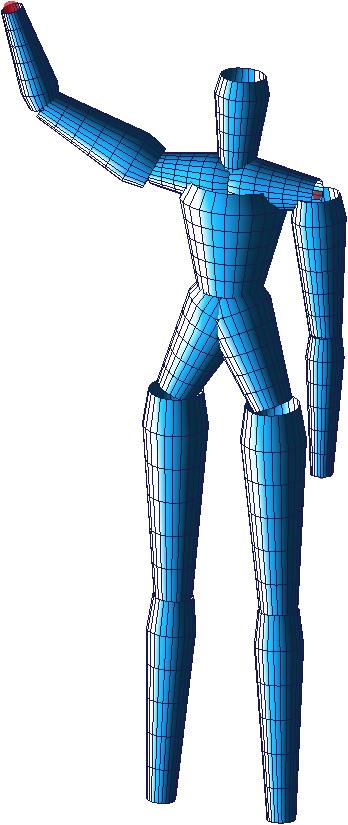
\includegraphics[height=2.3cm]{fig/body/others/weiz1.png} 
		\subcaption{Wave 1}
		\label{fig/body/others/e}
	\end{subfigure}
	\begin{subfigure}[t]{0.18\linewidth} \centering
		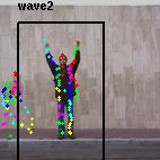
\includegraphics[height=2.3cm]{fig/body/others/weiz2.jpg} \\
		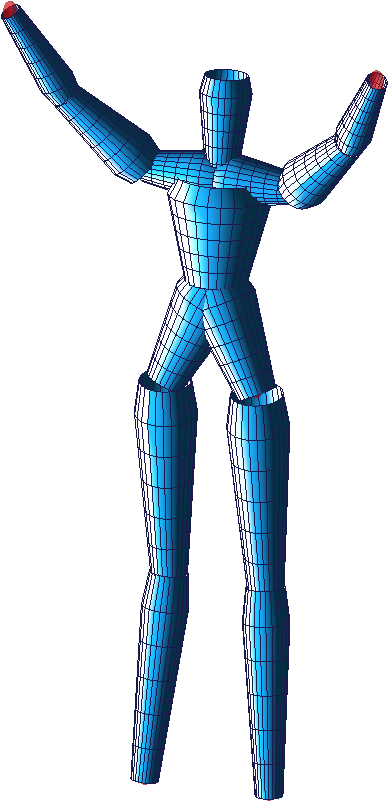
\includegraphics[height=2.3cm]{fig/body/others/weiz2.png} 
		\subcaption{Wave 2}
		\label{fig/body/others/f}
	\end{subfigure}
	\begin{subfigure}[t]{0.18\linewidth} \centering
		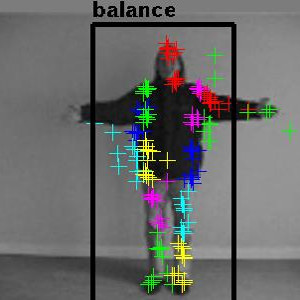
\includegraphics[height=2.3cm]{fig/body/others/ktherr.jpg} \\
		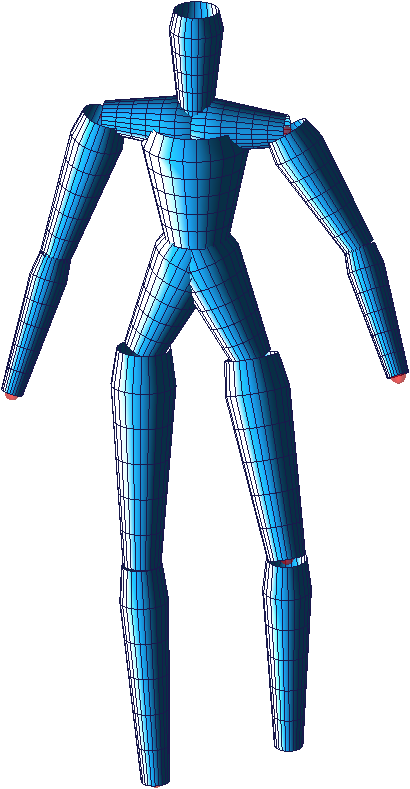
\includegraphics[height=2.3cm]{fig/body/others/ktherr.png} 
		\subcaption{Wave 2}
		\label{fig/body/others/g}
	\end{subfigure}
	\begin{subfigure}[t]{0.18\linewidth} \centering
		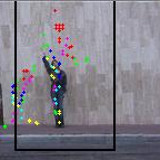
\includegraphics[height=2.3cm]{fig/body/others/weizerr.jpg} \\
		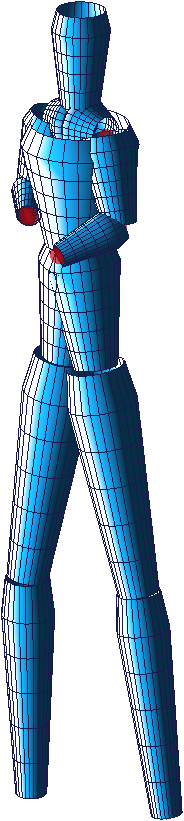
\includegraphics[height=2.3cm]{fig/body/others/weizerr.png} 
		\subcaption{Wave 1}
		\label{fig/body/others/h}
	\end{subfigure}
	\caption{Sample results obtained from applying the model trained from APE dataset to KTH (a--c, g) and Weizmann dataset (d--f, h).} 
	\label{fig/body/otherresults}
\end{figure}

